%%%%%%%%%%%%%%%%%%%%%%%%%%%%%%%%%%%%%%%%%
% baposter Landscape Poster
% LaTeX Template
% Version 1.0 (11/06/13)
%
% baposter Class Created by:
% Brian Amberg (baposter@brian-amberg.de)
%
% This template has been downloaded from:
% http://www.LaTeXTemplates.com
%
% License:
% CC BY-NC-SA 3.0 (http://creativecommons.org/licenses/by-nc-sa/3.0/)
%
%%%%%%%%%%%%%%%%%%%%%%%%%%%%%%%%%%%%%%%%%

%----------------------------------------------------------------------------------------
%	PACKAGES AND OTHER DOCUMENT CONFIGURATIONS
%----------------------------------------------------------------------------------------

\documentclass[landscape,a0paper,fontscale=0.285]{baposter} % Adjust the font scale/size here

\usepackage{graphicx} % Required for including images
\graphicspath{{../../media/}} % Directory in which figures are stored
\usepackage{algorithm, algorithmic}
\usepackage{ mathrsfs }
\usepackage{ dsfont }
\usepackage{amsmath} % For typesetting math
\usepackage{amssymb} % Adds new symbols to be used in math mode

\usepackage{booktabs} % Top and bottom rules for tables
\usepackage{enumitem} % Used to reduce itemize/enumerate spacing
\usepackage{palatino} % Use the Palatino font
\usepackage[font=small,labelfont=bf]{caption} % Required for specifying captions to tables and figures

\usepackage{amsthm}
%\usepackage{amsmath}
\usepackage[english]{babel}
 \theoremstyle{definition}
  \newtheorem{defn}{\protect\definitionname}
   \providecommand{\definitionname}{Definition}


\usepackage{multicol} % Required for multiple columns
\setlength{\columnsep}{1.5em} % Slightly increase the space between columns
\setlength{\columnseprule}{0mm} % No horizontal rule between columns

\usepackage{tikz} % Required for flow chart
\usetikzlibrary{shapes,arrows} % Tikz libraries required for the flow chart in the template

\newcommand{\compresslist}{ % Define a command to reduce spacing within itemize/enumerate environments, this is used right after \begin{itemize} or \begin{enumerate}
\setlength{\itemsep}{1pt}
\setlength{\parskip}{0pt}
\setlength{\parsep}{0pt}
}

\definecolor{lightblue}{rgb}{0.145,0.6666,1} % Defines the color used for content box headers
\definecolor{lightblue}{rgb}{0.145,0.6666,1}


%-------------------------------------------------------------------------------
%-------------------------------------------------------------------------------
% Ian's definitions
%-------------------------------------------------------------------------------
%-------------------------------------------------------------------------------

\newtheorem{theorem}{Theorem}
\newtheorem{corollary}{Corollary}
\newtheorem{lemma}{Lemma}
\newtheorem{mydef}{Definition}
\newtheorem{prop}{Proposition}
\newtheorem{claim}{Claim}

% Setting up macro shortcuts
\newcommand{\Exp}{\mathds{E}}
\newcommand{\Expk}{\mathds{E}_{k}}
\newcommand{\Prob}{\mathds{P}}
\newcommand{\Real}{\mathds{R}}
\newcommand{\Nat}{\mathbb{N}}
\newcommand{\Ind}{\mathds{1}}

\newcommand{\Xc}{\mathcal{X}}
\newcommand{\Yc}{\mathcal{Y}}
\newcommand{\Pc}{\mathcal{P}}
\newcommand{\Qc}{\mathcal{Q}}
\newcommand{\Fc}{\mathcal{F}}
\newcommand{\Gc}{\mathcal{G}}
\newcommand{\Rc}{\mathcal{R}}
\newcommand{\Sc}{\mathcal{S}}
\newcommand{\Ac}{\mathcal{A}}
\newcommand{\Mc}{\mathcal{M}}
\newcommand{\Tc}{\mathcal{T}}
\newcommand{\Vc}{\mathcal{V}}
\newcommand{\Dep}{ \Delta^H,\Delta^F,\mathcal{F},\epsilon }

\newcommand{\conf}{\mathcal{F}^d_t}

\newcommand{\vect}[1]{\boldsymbol{#1}}
\newcommand{\opt}{M^*}
\newcommand{\sampled}{{M_k}}
\newcommand{\Pstar}{P^{*}(\cdot \mid s_t, a_t)}
\newcommand{\Pk}{P_{k}(\cdot \mid s_t, a_t)}
\newcommand{\Pdiff}{(P_{k}-P^{*})(\cdot \mid s_t, a_t)}
\newcommand{\Rdiff}{(r_k-r^{*})(s_t, a_t)}
\newcommand{\optPol}{\mu^{*}}
\newcommand{\sampledPol}{\mu_{k}}
\newcommand{\bellmanSampled}{\mathcal{T}_{\mu_{k}(\cdot,i)}^{k}}
\newcommand{\bellmanTrue}{\mathcal{T}_{\mu_{k}(\cdot,i)}^{*}}
\newcommand{\bellmanSampledA}{\mathcal{T}_{\mu_{k}(\cdot,1)}^{k}}
\newcommand{\bellmanTrueA}{\mathcal{T}_{\mu_{k}(\cdot,1)}^{*}}
\newcommand{\vSampled}{V_{\mu_k, 1}^{k}}
\newcommand{\vSampledi}{V_{\mu_k, i}^{k}}
\newcommand{\vTrue}{V_{\tau, \mu_k}^{*}}


%-------------------------------------------------------------------------------
%-------------------------------------------------------------------------------
%-------------------------------------------------------------------------------
%-------------------------------------------------------------------------------


\begin{document}

\begin{poster}
{
headerborder=closed, % Adds a border around the header of content boxes
colspacing=1em, % Column spacing
bgColorOne=white, % Background color for the gradient on the left side of the poster
bgColorTwo=white, % Background color for the gradient on the right side of the poster
borderColor=lightblue, % Border color
headerColorOne=black, % Background color for the header in the content boxes (left side)
headerColorTwo=lightblue, % Background color for the header in the content boxes (right side)
headerFontColor=white, % Text color for the header text in the content boxes
boxColorOne=white, % Background color of the content boxes
textborder=roundedleft, % Format of the border around content boxes, can be: none, bars, coils, triangles, rectangle, rounded, roundedsmall, roundedright or faded
eyecatcher=true, % Set to false for ignoring the left logo in the title and move the title left
headerheight=0.1\textheight, % Height of the header
headershape=roundedright, % Specify the rounded corner in the content box headers, can be: rectangle, small-rounded, roundedright, roundedleft or rounded
headerfont=\Large\bf\textsc, % Large, bold and sans serif font in the headers of content boxes
%textfont={\setlength{\parindent}{1.5em}}, % Uncomment for paragraph indentation
linewidth=2pt % Width of the border lines around content boxes
}
%----------------------------------------------------------------------------------------
%	TITLE SECTION
%----------------------------------------------------------------------------------------
%
{
\includegraphics[height=4em]{logo}} % First university/lab logo on the left
{\bf\textsc{Near-Optimal Reinforcement Learning \\ \vspace{1mm} in Factored MDPs}\vspace{0.5em}} % Poster title
{\textsc{ Ian Osband and Benjamin Van Roy \hspace{12pt} Stanford University}} % Author names and institution
{
\includegraphics[height=4em]{logo}} % Second university/lab logo on the right

%----------------------------------------------------------------------------------------
%	Abstract
%----------------------------------------------------------------------------------------

\headerbox{Abstract}{name=abstract,column=0,row=0}{
Any reinforcement learning algorithm that applies to all MDPs will suffer $\Omega(\sqrt{SAT})$ regret on some MDP, where $T$ is the elapsed time and $S$ is the number of states and $A$ is the number of actions.
In many problems $S$ and $A$ are so huge that any regret bounds are totally impractical.

\vspace{2mm}

We show that, if the system is known to be a \emph{factored} MDP, it is possible to achieve regret that scales polynomially in the number of \emph{parameters} encoding the factored MDP, which may be exponentially smaller than $S$ or $A$.
We provide two algorithms that satisfy near-optimal regret bounds in this context: PSRL and UCRL-Factored.
\vspace{0.3em} % When there are two boxes, some whitespace may need to be added if the one on the right has more content
}


%----------------------------------------------------------------------------------------
%   Formulation
%----------------------------------------------------------------------------------------

\headerbox{Problem formulation}{name=forumulation,column=0,below=abstract,above=bottom}{

Learn to optimize a random finite horizon MDP $M$ in repeated finite episodes of interaction.

\begin{center}
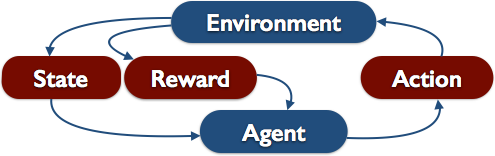
\includegraphics[width=0.8\linewidth]{basic_mdp}
\captionof{figure}{classic reinforcement learning setting}
\end{center}
\vspace{-15pt}

\begin{itemize}\compresslist
\item State space $\Sc$, action space $\Ac$
\item Rewards $r_t \sim R^M(s_t, a_t)$
\item Transitions $s_{t+1} \sim P^M(s_t, a_t)$
\item Epsiode length $\tau$, define $t_k := (k-1) \tau + 1$
\end{itemize}

For MDP $M$ and policy $\mu$, define a value function
\vspace{-3mm}
$$V^{M}_{\mu, i}(s) := \Exp_{M,\mu}\left[ \sum_{j=i}^{\tau} \overline{R}^M(s_j,a_j) \Big| s_i = s \right],$$

\vspace{-1mm} Define the regret in episode $k$ using $\mu_k$ on $M^*$
\vspace{-3mm}
$$\Delta_k := \sum_{\Sc} \rho(s) \bigg(\underbrace{V^{M^*}_{\mu^*, 1}(s)}_{\textcolor{red}{\text{optimal value}}} - \underbrace{V^{M^{*}}_{\mu_k, 1}(s)}_{\textcolor{red}{\text{actual value}}}\bigg)$$

\vspace{-1mm} And finally
${\rm Regret}(T, \pi, M^*) := \sum_{k=1}^{\lceil T/\tau \rceil} \Delta_k$.

\vspace{2mm}
Naive exploration such as Boltzman or $\epsilon$-greedy can lead to exponential regret.
Good performance requires balancing \textcolor{red}{\textbf{exploration vs exploitation}}.
Carefully designed optimism or posterior sampling can learn quickly in factored MDPs.
}

%----------------------------------------------------------------------------------------
%	Factored MDPs
%----------------------------------------------------------------------------------------

\headerbox{Factored MDPs}{name=factored,column=1,row=0}{
MDP with conditional independence structure.

\begin{center}
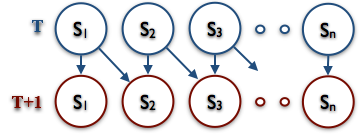
\includegraphics[width=0.6\linewidth]{transitions}
\captionof{figure}{a graphical model for transitions.}
\end{center}

\vspace{-4mm}
\begin{mydef}[Scope operation for factored sets]
\hspace{0.000000001mm} \newline
For any $\Xc = \Xc_1 \times .. \times \Xc_n$ and $Z \subseteq \{1,2,..,n\}$ define $\Xc[Z] := \bigotimes\limits_{i \in Z} \Xc_i$ and elements $x[Z] \in \Xc[Z]$.
\end{mydef}

\vspace{-4mm}
\begin{mydef}[Factored reward functions]
\hspace{0.000000001mm} \newline
The reward function $r$ is factored over $\Sc \times \Ac = \Xc = \Xc_1 \times .. \times \Xc_n $ with scopes $Z_1, .. Z_l \iff$
\vspace{-3mm}
$$ \Exp [ r(x) ] = \sum_{i=1}^l \Exp\big[ r_i(x[Z_i]) \big] \ \ {\rm and \ each} \ r_i \ {\rm observed} $$
\end{mydef}

\vspace{-4mm}
\begin{mydef}[ Factored transition functions]
\hspace{0.000000001mm} \newline
The transition function $P$ is factored over $\Sc \times \Ac = \Xc = \Xc_1 \times .. \times \Xc_n$ and $\Sc = \Sc_1 \times .. \times \Sc_m$ with scopes  $Z_1, .. Z_m \iff$
\vspace{-3mm}
$$ P(s | x) = \prod_{i=1}^m P_i \left( s[i] \ \bigg\vert \ x[Z_i] \right) $$
\end{mydef}
\vspace{1mm}
}

%----------------------------------------------------------------------------------------
%   Main Results
%----------------------------------------------------------------------------------------

\headerbox{Main results}{name=main,column=1,below=factored, above=bottom}{
\vspace{-1mm}
For $M^*$ factored with known graphical structure as above then for PSRL and UCRL-Factored
\vspace{-2mm}
\textcolor{red}{$$ \mathbf{{\rm \textbf{Regret}(T, M^*)} = \tilde{O}}
\left( \Xi \sum_{j=1}^m  \sqrt{|\Xc[Z^P_j]| \ |\Sc_j| \ T } \right). $$}

\vspace{-2mm}
Here $\Xi$ is a measure of MDP connectedness for each algorithm, expected span $\Exp[\Psi]$ for PSRL and diameter $D$ for UCRL-Factored.

\vspace{1mm}
PSRL's bounds are tighter since $\Psi(M) \le D(M)$ and may be exponentially smaller.
However, UCRL-Factored holds with high probability for any $M^*$ not just in expectation over the prior.

\vspace{1mm}
\textbf{Key point:} For $m$ independent components with $S$ states and $A$ actions $ \color{red}{= \tilde{O}(mS\sqrt{AT})}$ and close to
\vspace{-3mm}
$$\color{blue}{\underbrace{m\sqrt{SAT)}}_{\text{factored MDP lower bound}}}
 \ll \color{green}{\underbrace{\sqrt{(SA)^m T}}_{\text{general MDP lower bound}}}.$$
}

%----------------------------------------------------------------------------------------
%	Posterior sampling
%----------------------------------------------------------------------------------------

\headerbox{Posterior Sampling}{name=posterior,column=2,span=1,row=0}{
For each episode $k$:
\begin{enumerate}
\item Sample an MDP from the posterior distribution for the true MDP: $M_k \sim \phi(\cdot | H_t)$.
\item Use policy $\mu_k \in \underset{\mu, M}{\arg\max} V^{M_k}_\mu$.
\end{enumerate}

\textbf{Proof sketch:}
\vspace{-4mm}
\begin{eqnarray*}
    \Delta_k &=&  V^*_{*,1}(s) - V^*_{k,1}(s)\\
     &=& \underbrace{\big( V^k_{k,1}(s) - V^*_{k,1}(s) \big)}_{\text{Imagined - Actual}}
     + \underbrace{\big(V^*_{*,1}(s) - V^k_{k,1}(s) \big)}_{\Exp[\cdot] = 0}
\end{eqnarray*}
We can decompose this into Bellman error:
\vspace{-4mm}
\begin{equation*}
    V^k_{k,1} - V^*_{k,1} =
    \underbrace{\sum_{i=1}^\tau \left( \Tc^k_{k,i} - \Tc^*_{k,i} \right) V^k_{k,i+1}}_{B := \text{Bellman error}}
    + \underbrace{ \sum_{i=1}^\tau d_{t_k+1}}_{\Exp=0 \text{ martingale}}.
\end{equation*}
We can now use the H\"{o}lder inequality to bound:
\vspace{-3mm}
\begin{equation*}
\label{eq: err sums}
    B \le \sum_{i=1}^\tau \bigg\{
    \underbrace{|\overline{R}^k - \overline{R}^* |}_{\text{reward error}}
    + \frac{1}{2} \underbrace{\Psi_k}_{\text{MDP span}} \underbrace{\|P^k - P^* \|_1}_{\text{transition error}}
    \bigg\}
\end{equation*}

We conclude the proof by upper bounding these deviations by maximum possible within $\Mc_k$.
Concentration inequalities allows us to build tight $\Mc_k$ that contain $M^*$ with high probability.

}

%----------------------------------------------------------------------------------------
%   Optimism
%----------------------------------------------------------------------------------------

\headerbox{Optimsim}{name=optimism,column=3,span=1,row=0}{
For each episode $k$:
\begin{enumerate}
\item Form $\mathcal{M}_k$ subset of MDPs $M$ that are statistically plausible given the data.
\vspace{-2mm}
\item Use policy $\mu_k \in \underset{\mu}{\arg\max} \left\{ \underset{M \in \Mc_k}{\max} V^M_\mu(s) \right\}$.
\end{enumerate}

\textbf{Proof sketch:}
\vspace{-4mm}
\begin{eqnarray*}
    \Delta_k &=&  V^*_{*,1}(s) - V^*_{k,1}(s)\\
     &=& \underbrace{\big( V^k_{k,1}(s) - V^*_{k,1}(s) \big)}_{\text{Imagined - Actual}}
     + \underbrace{\big(V^*_{*,1}(s) - V^k_{k,1}(s) \big)}_{\le 0 \text{ by optimism}}
\end{eqnarray*}

\vspace{-2mm}

Then follow the analysis per posterior sampling.
}



%----------------------------------------------------------------------------------------
%	CONTACT INFORMATION
%----------------------------------------------------------------------------------------

\headerbox{Contact Information}{name=contact,column=3,above=bottom}{ % This block is as tall as the references block

\begin{description}\compresslist
\item[Web] www.stanford.edu/$\sim$iosband
\item[Email] iosband@stanford.edu
%\item[Phone] +1 (000) 111 1111
\end{description}
}

%----------------------------------------------------------------------------------------
%   REFERENCES
%----------------------------------------------------------------------------------------

\headerbox{References}{name=references,aligned=contact,column=2,above=bottom}{

%\renewcommand{\section}[2]{\vskip 0.05em} % Get rid of the default "References" section title
%\nocite{*} % Insert publications even if they are not cited in the poster
%\small{ % Reduce the font size in this block
%\bibliographystyle{unsrt}
%\bibliography{sample} % Use sample.bib as the bibliography file
%}
Please see the full paper: \\
http://arxiv.org/abs/1403.3741
}

%----------------------------------------------------------------------------------------
%	ANALYSIS
%----------------------------------------------------------------------------------------

\headerbox{Key lemma}{name=lemma,column=2,span=1,row=0, below=posterior, above=references}{
For any $P,\tilde{P}$ factored transition functions we may bound their L1 distance by the sum of the differences of their factorizations:
$$ \| P(x) - \tilde{P}(x) \|_1 \le \sum_{i=1}^m \|P_i(x[Z_i]) - \tilde{P}_i(x[Z_i]) \|_1 $$

\textbf{Proof sketch:}

For any $ \alpha_1, \alpha_2, \beta_1, \beta_2 \in [0,1]:$
\vspace{-2mm}
$$ | \alpha_1 \alpha_2 - \beta_1 \beta_2 | \le \alpha_2 \left| \alpha_1 - \beta_1 \right| + \beta_1 \left| \alpha_2 - \beta_2 \right|.$$

\vspace{-1mm}
Repeat this argument for desired result.

}

\headerbox{Example}{name=example,column=3,span=1,row=0, below=optimism}{
Production line with 100 machines, each with 3 states and 3 actions.
Each machine generates some revenue we want to maximize jointly.

\begin{center}
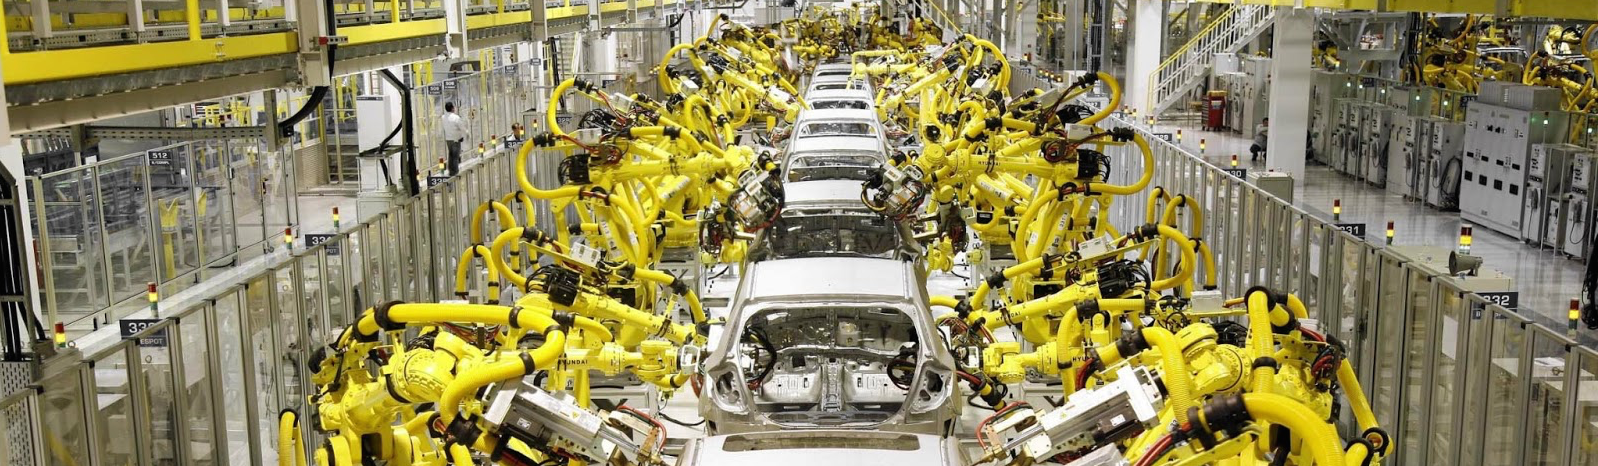
\includegraphics[width=0.6\linewidth]{productionLine2}
\captionof{figure}{automated production line}
\end{center}
\vspace{-12pt}

\vspace{1mm}
This MDP has state $s = (s_1, .. ,s_{100})$ and action $a = (a_1, .. ,a_{100})$.
Here $S = A = 3^{100} \simeq 10^{50}$, so even a maximally efficient general-purpose learner would have regret $\Omega(\sqrt{SAT}) \simeq \color{red}{10^{50}\sqrt{T}}$.

\vspace{2mm}
If over a single timestep, each machine depends directly only upon its neighbours then this becomes a factored MDP.
Now $|\Xc[Z^P_j]| \le 3^3$ and $|S_j| \le 3$ for each machine $j$.

\vspace{2mm}
We exploit this graphical structure for exponentially smaller regret $\simeq 100 \sqrt{3^3 \times 3 \times T} \simeq \color{red}{10^3 \sqrt{T}}$.
\vspace{0.1mm}
}

\headerbox{Key takeaway}{name=example,column=3,span=1,row=0, below=example, above=references}{
\textbf{Our regret bounds scale with the number of \\ parameters, not the number of states.}
}





%----------------------------------------------------------------------------------------

\end{poster}

\end{document}
